\documentclass[11pt,a4paper]{amsart}

\usepackage[T1]{fontenc}
\usepackage[utf8]{inputenc}
\usepackage{lmodern}
\usepackage[a4paper,margin=29mm]{geometry}
\usepackage{amsmath,amssymb,amsthm,mathtools}
\usepackage{microtype}
\usepackage{enumitem}
\usepackage[hidelinks]{hyperref}
\usepackage{subcaption}
\usepackage[
    style=numeric,
    sorting=nty,
    maxnames=99,
    maxalphanames=5,
    natbib=true,
    backend=biber,
    sortcites]{biblatex}
\usepackage{todonotes}
\usepackage{xcolor}
\newcommand{\fr}[1]{{\color{red} #1}}

\bibliography{references}


\hypersetup{
  pdftitle={Real-valued Jordan curves and nonreal limiting spectra of banded Toeplitz matrices},
  pdfauthor={F. Rohner, C. Thalhammer},
  pdfsubject={Explicit counterexamples to a Jordan-curve criterion for real Toeplitz limiting spectra},
  pdfkeywords={Toeplitz matrices, limiting spectrum, Laurent polynomial, Jordan curve, Schmidt-Spitzer theorem}
}

\newtheorem{theorem}{Theorem}[section]
\newtheorem{proposition}[theorem]{Proposition}
\newtheorem{lemma}[theorem]{Lemma}
\newtheorem{corollary}[theorem]{Corollary}
\theoremstyle{remark}
\newtheorem{remark}[theorem]{Remark}
\numberwithin{equation}{section}
\newtheorem{conjecture}[theorem]{Conjecture}

\newcommand{\C}{\mathbb C}
\newcommand{\R}{\mathbb R}
\newcommand{\N}{\mathbb N}
\newcommand{\ii}{\mathrm i}
\DeclareMathOperator{\wind}{wind}
\DeclareMathOperator{\spec}{spec}
\DeclareMathOperator{\Rea}{Re}
\DeclareMathOperator{\Ima}{Im}

\title[Jordan curves and Toeplitz limiting spectra]{Real-valued Jordan curves and nonreal limiting spectra of banded Toeplitz matrices}
\author[F. Rohner]{Fabian Rohner}
\author[C. Thalhammer]{Clemens Thalhammer}
\date{September 7, 2026}
\subjclass[2020]{15B05, 47B36}
\keywords{Banded Toeplitz matrices, limiting spectrum, Laurent polynomials, Jordan curves, equal-modulus roots}

\begin{document}

\begin{abstract}
We construct Laurent polynomials that are real-valued on a Jordan curve
  surrounding the origin but whose banded Toeplitz matrices have nonreal
  limiting spectrum. This refutes the weakest surviving form of a conjecture
  of Shapiro and \v{S}tampach.
\end{abstract}

\maketitle

\section{Introduction and main results}
\label{sec:intro}

Let
\begin{equation}
 b(z)=\sum_{k=-r}^{s}b_kz^k,
 \qquad r,s\geq1,\qquad b_{-r}b_s\neq0,
 \label{eq:symbol}
\end{equation}
be a Laurent polynomial, and let
\[
 T_n(b)=(b_{i-j})_{i,j=1}^{n}
\]
be its finite Toeplitz sections. We are interested in the limiting spectrum
\begin{equation}
 \Lambda(b)=\{\lambda \in \C: \lim_{n\rightarrow\infty}\operatorname{dist}(\lambda, T_n(b))=0\}.
 \label{eq:limiting-spectrum}
\end{equation}
For each \(\lambda\in\C\), denote the roots of
\begin{equation}
 z^r\bigl(b(z)-\lambda\bigr)=0
 \label{eq:root-polynomial}
\end{equation}
by \(z_1(\lambda),\ldots,z_{r+s}(\lambda)\), repeated according to multiplicity and ordered so that
\[
 0<|z_1(\lambda)|\leq\cdots\leq|z_{r+s}(\lambda)|.
\]
The following characterisation of the limiting spectrum is classical \cite{schmidt1960toeplitz}.
\begin{theorem}\label{thm: SchmidtSpitzer}
    Let $b$ be a Laurent polynomial as defined in \ref{eq:symbol}. Then it holds that
    \begin{equation}
        \begin{aligned}
            \Lambda(b) &=\bigcap_{r>0}\sigma(T(b(rz))\\
            &=\{\lambda \in \C: \lvert z_r(\lambda)\lvert=\rvert z_{r+1}(\lambda)\lvert\}
        \end{aligned}
    \end{equation}
\end{theorem}

An important question is when the limiting spectrum is real-valued. While this is trivially the case for self-adjoint operators, it has also been numerically observed for a wide range of non-self-adjoint Toeplitz matrices.

\begin{conjecture}\label{conj: Reality}
    Let $b$ be a Laurent polynomial as in \eqref{eq:symbol}. The following are equivalent
    \begin{enumerate}
        \item\label{conj: Reality1} $\Lambda(b)\subset\R$,
        \item\label{conj: Reality2} the set $b^{-1}(\R)$ contains a Jordan curve with the origin in its interior,
        \item\label{conj: Reality3} $\sigma(T_n(b))\subset \R$ for all $n\in\N$.
    \end{enumerate}
\end{conjecture}

The above conjecture was first asserted as a Theorem in \cite{shapiro2019non}, unfortunately the proof was later discovered to be erroneous \cite{Shapiro2023} and remains the subject of active research \cite{de2026mathematical,townsend2026openproblemsnla}. The implication $\eqref{conj: Reality1}\implies\eqref{conj: Reality2}$ remains proven as it was unaffected by the error and is also known to hold in the case of matrix-valued symbols \cite{giandinoto2024reality}. Common belief was that the implication $\eqref{conj: Reality2}\implies\eqref{conj: Reality3}$, or at least the weaker result $\eqref{conj: Reality2}\implies\eqref{conj: Reality1}$ would still hold. The former has recently been disproven in \cite{colbrook2026sp06}, but the later direction remained open until now.

In this paper, we provide two surprisingly simple counterexamples to $\eqref{conj: Reality2}\implies\eqref{conj: Reality1}$ (and consequently also the stronger claim $\eqref{conj: Reality2}\implies\eqref{conj: Reality3}$). The main result, Theorem \ref{thm:main}, shows that the open part Conjecture \ref{conj: Reality} is false, even when restricting to symbols with real-valued coefficients. 


\begin{theorem}
\label{thm:main}
Define
\begin{equation}
 h(z)=z^2+97z+103-\frac{10201}{z},
 \qquad b(z)=h(z)^2.
 \label{eq:h-b}
\end{equation}
Then \(b\) has real Laurent coefficients, with \(r=2\) and \(s=4\), and the following statements hold.
\begin{enumerate}[label=\textup{(\roman*)},leftmargin=2.1em]
\item There is a real-analytic Jordan curve \(\gamma\subset\C\setminus\{0\}\) satisfying
\[
 \wind(\gamma,0)=1,
 \qquad b(\gamma)=[-4000000,0].
\]
\item Set
\begin{equation}
 \rho=\frac{101}{\sqrt{97}},\qquad
 L=\frac{20192}{97},\qquad
 \lambda_0=L^2.
 \label{eq:constants}
\end{equation}
In a neighborhood of \(\lambda_0\), the set \(\Lambda(b)\) is a regular real-analytic arc transverse to the real axis. It has a parametrization \(\lambda(t)\), for real \(t\) near \(0\), such that
\begin{equation}
 \lambda(t)=\lambda_0+\ii C t+O(t^2),
 \qquad C=\frac{2L\rho(97^2-\rho^2)}{97}>0.
 \label{eq:arc-expansion}
\end{equation}
All six roots of \(z^2(b(z)-\lambda)\) are simple throughout a sufficiently small neighborhood of \(\lambda_0\).
\end{enumerate}
Consequently, \(\Lambda(b)\not\subset\R\).
\end{theorem}
\begin{figure}[htbp]
     \centering
     % --- FIRST ROW ---
     \begin{subfigure}[b]{0.45\textwidth}
         \centering
         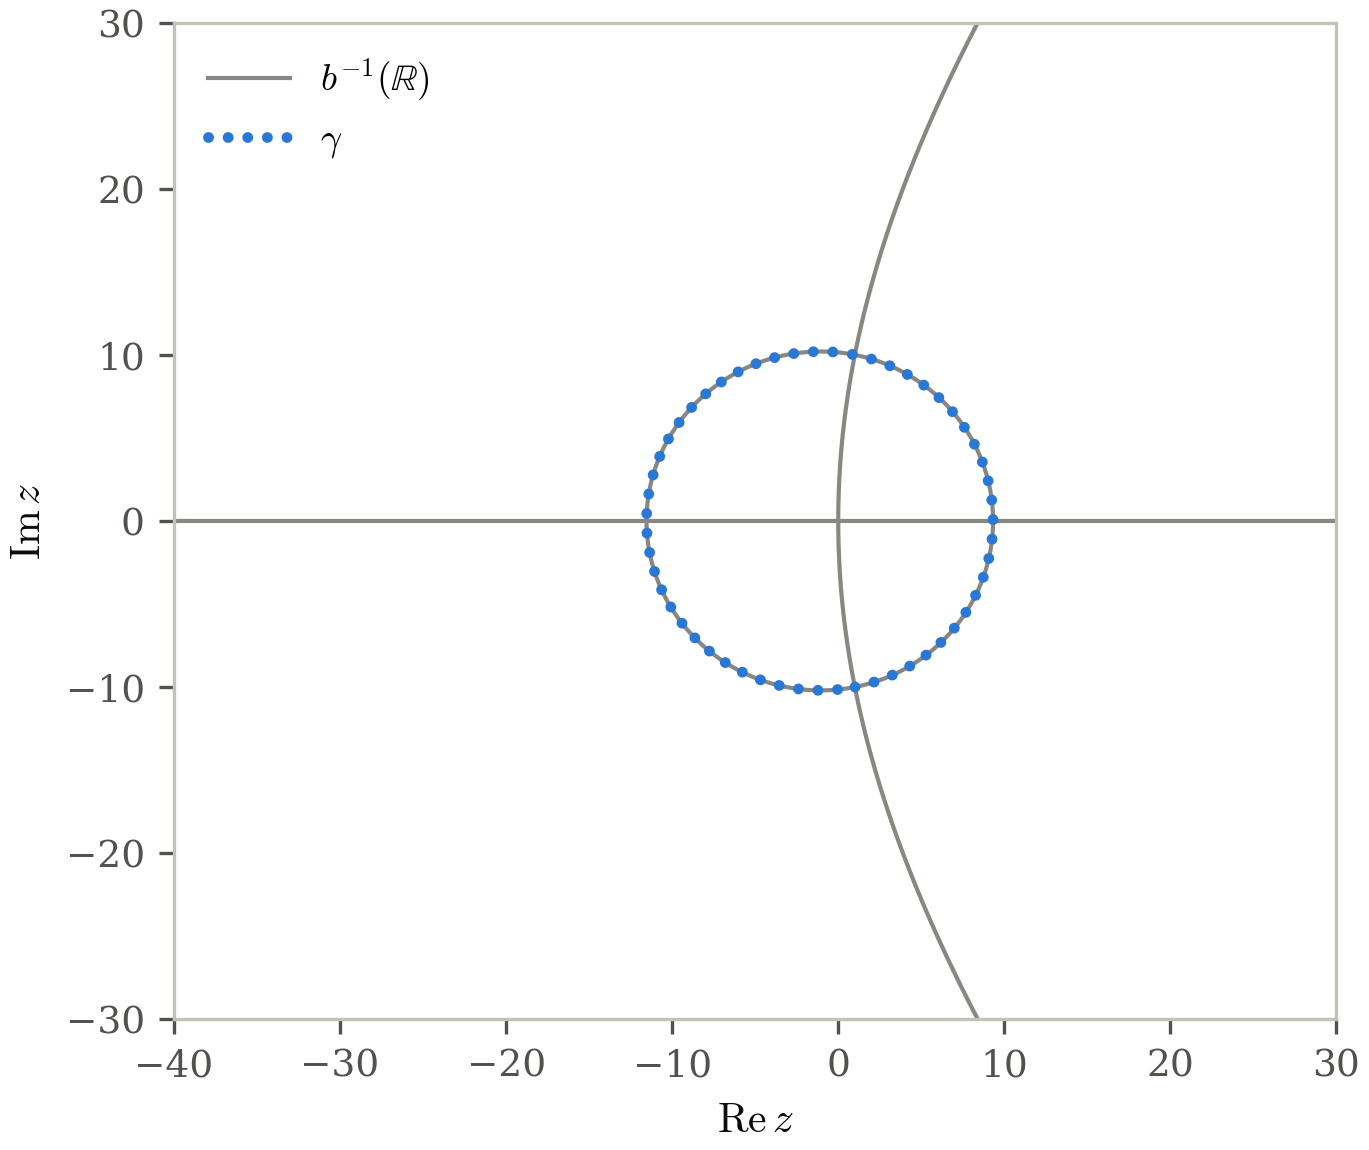
\includegraphics[width=\textwidth]{figures/fig_preimage_real.png}
         \caption{Preimage of $\R$}
         \label{fig:Main1}
     \end{subfigure}
     \hfill
     \begin{subfigure}[b]{0.45\textwidth}
         \centering
         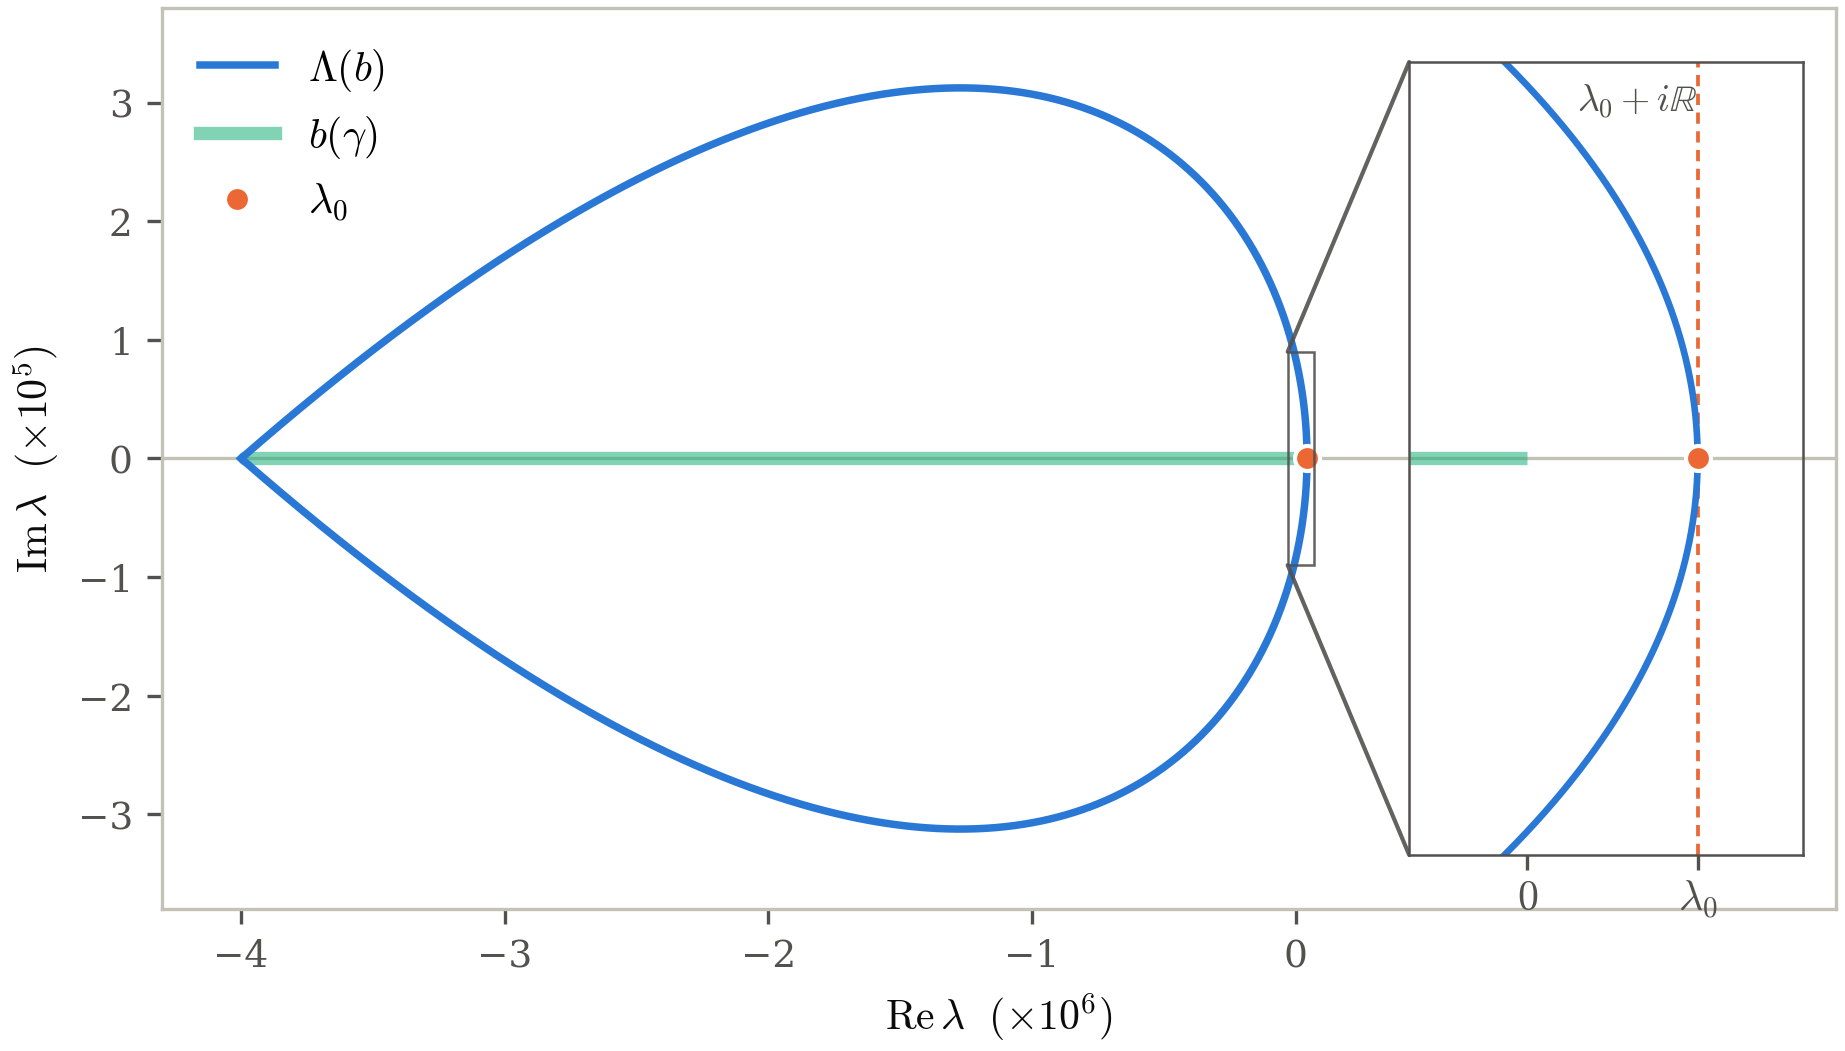
\includegraphics[width=\textwidth]{figures/fig_limiting_spectrum.png}
         
         \caption{Limiting spectrum}
         \label{fig:Main2}
     \end{subfigure}

     \vspace{1em} % Adds some vertical spacing between the rows

     % --- SECOND ROW ---
     \begin{subfigure}[b]{0.45\textwidth}
         \centering
         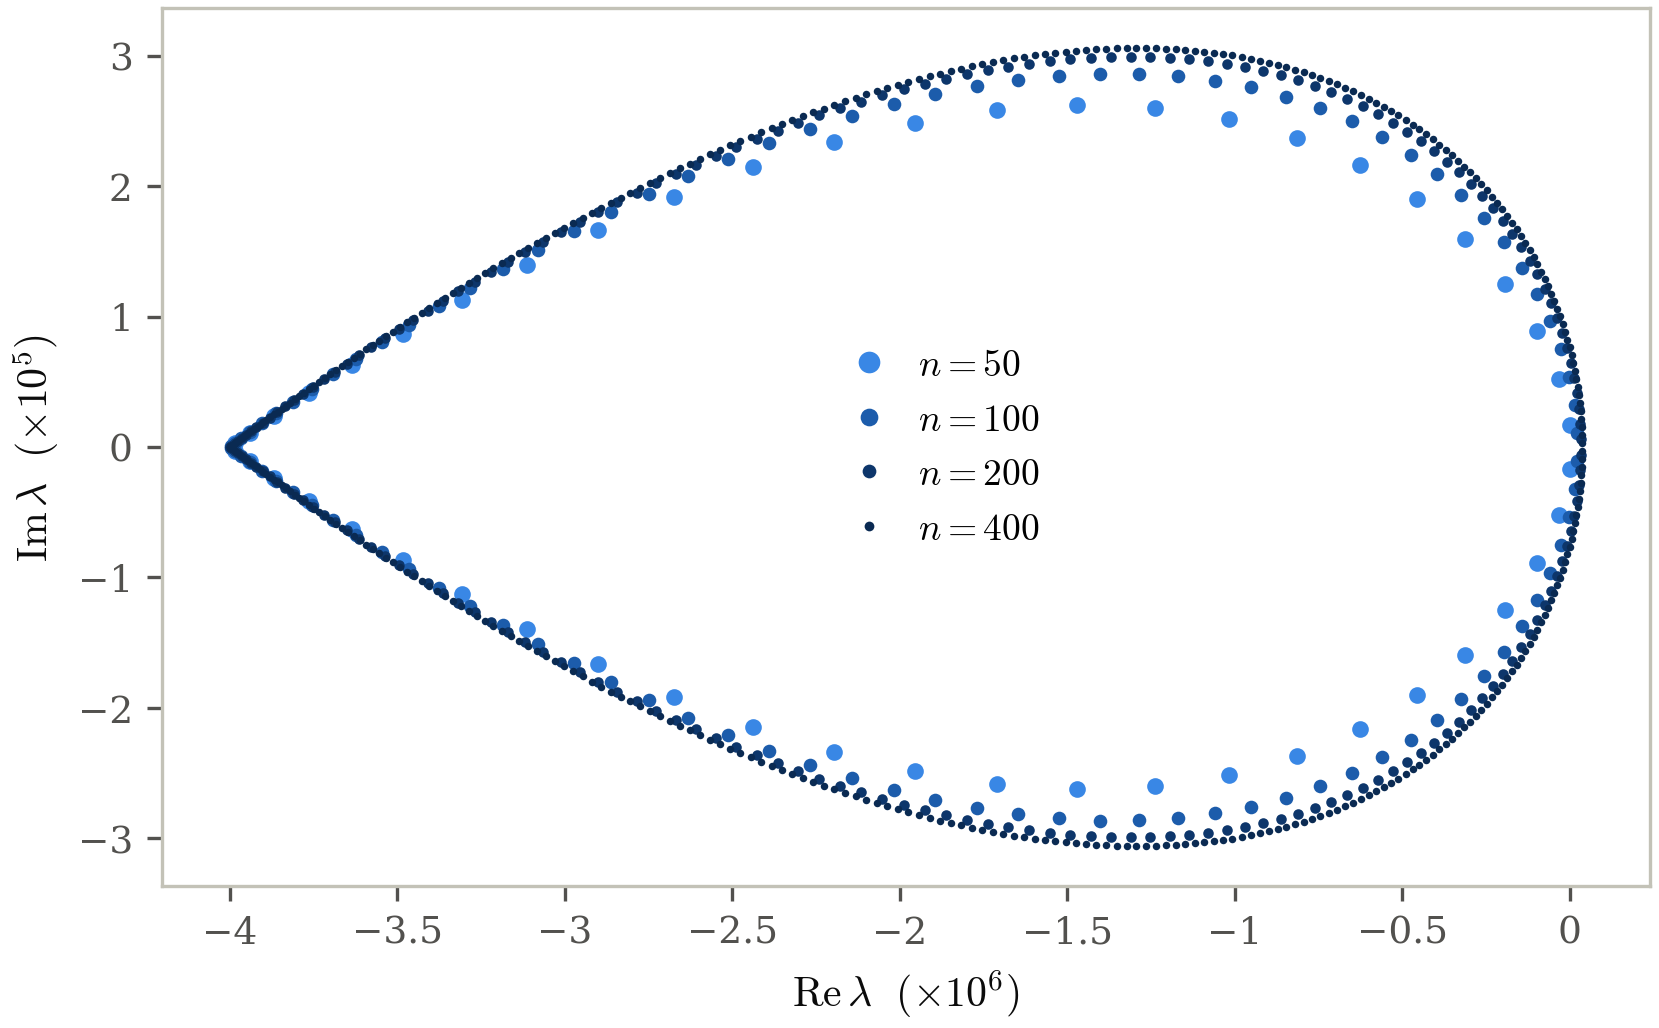
\includegraphics[width=\textwidth]{figures/fig_finite_spectra.png}
         \caption{Finite section spectra}
         \label{fig:single_resonator_linear3}
     \end{subfigure}
     
     \caption{Preimage of $\R$ and Limiting Spectrum for $b$ as in Theorem \ref{thm:main}}
     \label{fig:Main}
\end{figure}


A second example, proved in Section~\ref{sec:complex}, has \(r=1\) and \(s=2\):
\begin{equation}
 a(z)=\frac{10201}{z}+97z+\ii(103-z^2).
 \label{eq:a-intro}
\end{equation}
It is real-valued on the rotated curve \(\ii\gamma\), but
\begin{equation}
 \frac{20192}{97}\ii\in\Lambda(a).
 \label{eq:explicit-nonreal}
\end{equation}

The remainder of the paper is structured as follows: The curve $\gamma$ is constructed in Section \ref{sec:curve}. Section \ref{sec:real-spectrum} establishes the root ordering and non-reality of the spectrum. In Section \ref{sec:complex} the simpler counterexample \eqref{eq:a-intro} is discussed in more detail.



\section{Construction of \texorpdfstring{$\gamma$}{γ}}
\label{sec:curve}

We first construct
a Jordan curve on which \(h\) is purely imaginary. Squaring \(h\) will then make the symbol real on the same curve.

\begin{lemma}
\label{lem:rouche}
For every \(t\in[-2000,2000]\), the polynomial
\begin{equation}
 P_t(z)=z\bigl(h(z)-\ii t\bigr)
       =z^3+97z^2+(103-\ii t)z-10201
 \label{eq:Pt}
\end{equation}
has exactly two roots in \(|z|<30\), counted with multiplicity, and no root on \(|z|=30\).
\end{lemma}

\begin{proof}
Compare \(P_t\) with
\[
 Q_t(z)=100z^2-\ii tz-10000.
\]
The roots of \(Q_t\) are
\[
 \frac{\ii t\pm\sqrt{4000000-t^2}}{200},
\]
and both have modulus \(10\) for $t\in[-2000,2000]$. By factoring $Q_t$, we obtain on \(|z|=30\),
\[
 |Q_t(z)|\geq100(30-10)^2=40000.
\]
On the same circle,
\begin{align*}
 |P_t(z)-Q_t(z)|
  &=|z^3-3z^2+103z-201|\\
  &\leq30^3+3\cdot30^2+103\cdot30+201\\
  &=32991<40000.
\end{align*}
Rouch\'e's theorem gives the asserted root count, and the strict inequality excludes roots on the circle.
\end{proof}

\begin{proposition}
\label{prop:curve}
The set
\begin{equation}
 \gamma=\{z\in\C:|z|<30,\ h(z)\in\ii[-2000,2000]\}
 \label{eq:gamma}
\end{equation}
is a real-analytic Jordan curve. Its bounded interior contains \(0\), and
\[
 h(\gamma)=\ii[-2000,2000],\qquad
 b(\gamma)=[-4000000,0].
\]
\end{proposition}

\begin{proof}
The critical points of \(h\) are obtained from
\begin{equation}
 z^2h'(z)=2z^3+97z^2+10201
        =(2z+101)\bigl((z-1)^2+100\bigr).
 \label{eq:critical-factor}
\end{equation}
They are \(1+10\ii\), \(1-10\ii\), and \(-101/2\). Their critical values are
\begin{equation}
 h(1+10\ii)=2000\ii,\quad
 h(1-10\ii)=-2000\ii,\quad
 h(-101/2)=-\frac{8173}{4}.
 \label{eq:critical-values}
\end{equation}
Each is a simple critical point: \(h'\) has a simple zero there.

For \(-2000<t<2000\), every root of \(P_t\) is simple. Indeed, \(P_t(0)\neq0\), and a multiple root would satisfy \(h(z)=\ii t\) and \(h'(z)=0\), contrary to \eqref{eq:critical-values}. By Lemma~\ref{lem:rouche}, exactly two roots lie in \(|z|<30\). They can be labeled as locally real-analytic functions
\[
 \alpha(t),\ \beta(t),\qquad -2000<t<2000.
\]


% For clarity, this continuation is along a real interval, not through a branch point. The implicit function theorem provides local branches; simplicity and the absence of roots on \(|z|=30\) allow their continuation on each compact subinterval. Since the parameter interval is simply connected, the two branches may be labeled consistently on the whole open interval.

At the endpoints there are exact factorizations
\begin{equation}
 P_{\pm2000}(z)
   =\bigl(z-(1\pm10\ii)\bigr)^2\bigl(z+99\pm20\ii\bigr).
 \label{eq:endpoint-factors}
\end{equation}
The third root has modulus \(101\). Thus the only root inside \(|z|<30\) at either endpoint is the indicated double root. Continuity of polynomial roots, together with Lemma~\ref{lem:rouche}, yields continuous extensions of both branches with
\begin{align*}
 \alpha(-2000)=\beta(-2000)&=1-10\ii,\\
 \alpha(2000)=\beta(2000)&=1+10\ii.
\end{align*}

Each extended branch is injective. For example, equality \(\alpha(t_1)=\alpha(t_2)\) implies
\[
 \ii t_1=h(\alpha(t_1))=h(\alpha(t_2))=\ii t_2.
\]
An intersection between the two branches likewise forces equality of the parameters. At an interior parameter the two roots are distinct, so the branches have only their two endpoints in common. Their union is therefore a Jordan curve, and Lemma~\ref{lem:rouche} shows that this union is exactly \eqref{eq:gamma}.

Away from the two endpoints, the curve is real-analytic by the implicit
function theorem, since $h'\neq0$ there. To examine an endpoint, \fix one of the two signs and set $c = 1\pm10\ii$, so that $h(c) = \pm 2000\ii$. As $c$ is a simple critical point,
\[
  h(z)-h(c )=(z-c)^2 g(z)
\]
with $g$ holomorphic near $c$ and $g(c)\neq0$. Choosing a holomorphic branch
of $\sqrt{g}$ on a disc around $c$, set $\zeta(z):=(z-c)\sqrt{g(z)}$. Then
$\zeta(c)=0$, $\zeta'(c)=\sqrt{g(c)}\neq0$, and
\[
  h(z)-h(c)=\zeta(z)^2 ,
\]
so $\zeta$ maps a neighbourhood of $c$ conformally \cite[Corollary 2]{ahlfors1979complex} onto a neighbourhood of
$0$, in which $h$ becomes the map $\zeta\mapsto h(c)+\zeta^2$. Near $c$ the curve is the preimage under $h$ of a sufficiently short one-sided segment $h(c)\mp \ii [0,\varepsilon)$, with $\varepsilon>0$.
In the \(\zeta\)-coordinate, this preimage is the straight-line segment
\[
    e^{\mp\mathrm i\pi/4} \bigl(-\sqrt{\varepsilon},\sqrt{\varepsilon}\bigr),
\]
symmetric about $0$, whose two halves correspond to the two root branches that coalesce at $c$.
%a segment of $h(c)\mp i[0,4000]$ symmetric around $h(c)$. 
% Under $\zeta\mapsto h(c)+\zeta^2$ this segment has as preimage a segment of straight line
% $e^{\mp i\pi/4}\,\mathbb{R}$ symmetric around $0$, the two half-lines corresponding to the two root
% branches that coalesce at $c$. 
The curve near $c$ is therefore the image of a
straight line under the conformal map $\zeta^{-1}$, hence a regular
real-analytic arc through $c$.



The curve avoids \(0\), since \(P_t(0)=-10201\) for every \(t\). Let \(D\) be its bounded interior. If \(0\notin D\), then \(h\) would be holomorphic on a neighborhood of \(\overline D\), with \(\Rea h=0\) on \(\partial D\). The maximum and minimum principles for \(\Rea h\) would give \(\Rea h=0\) throughout \(D\). The open mapping theorem would then force \(h\) to be constant, a contradiction. Hence \(0\in D\), and positive orientation gives \(\wind(\gamma,0)=1\).

Every parameter in the segment occurs on either branch, so \(h(\gamma)=\ii[-2000,2000]\). Squaring proves the statement about \(b(\gamma)\).
\end{proof}

\section{The real-coefficient example}
\label{sec:real-spectrum}

Expanding \eqref{eq:h-b} gives
\begin{equation}
 \begin{split}
 b(z)={}&z^4+194z^3+9615z^2-420z-1968385\\
        &-\frac{2101406}{z}+\frac{104060401}{z^2}.
 \end{split}
 \label{eq:b-expanded}
\end{equation}
In particular, its pole order is \(2\), so the middle-root condition is
\(|z_2(\lambda)|=|z_3(\lambda)|\). Recall \(\rho,L,\lambda_0\) from \eqref{eq:constants}; they satisfy
\begin{equation}
 \rho^2=\frac{10201}{97},\qquad L=103+\rho^2,
 \qquad 10<\rho<11,\quad 208<L<209.
 \label{eq:rho-L}
\end{equation}

\subsection{Exact root ordering at a real spectral parameter}

\begin{lemma}
\label{lem:ordering}
All six roots of \(z^2(b(z)-\lambda_0)\) are simple. Their moduli satisfy
\begin{equation}
 |z_1(\lambda_0)|<\rho
 =|z_2(\lambda_0)|=|z_3(\lambda_0)|
 <|z_4(\lambda_0)|<|z_5(\lambda_0)|<|z_6(\lambda_0)|.
 \label{eq:ordering}
\end{equation}
The two roots of modulus \(\rho\) are \(\rho\) and \(-\rho\).
\end{lemma}

\begin{proof}
Since \(\lambda_0=L^2\), the equation \(b(z)=\lambda_0\) splits into \(h(z)=L\) and \(h(z)=-L\). For the first equation,
\begin{equation}
 z(h(z)-L)
  =z^3+97z^2-\rho^2z-10201
  =(z+97)(z^2-\rho^2).
 \label{eq:h-L-factor}
\end{equation}
Its roots are \(-97,-\rho,\rho\).

For the second equation, let
\[
 q(z)=z(h(z)+L)=z^3+97z^2+(103+L)z-10201.
\]
The following signs are exact:
\begin{align*}
 q(-97)&=-194L<0, & q(-30)&=47009-30L>0,\\
 q(-\rho)&=-2L\rho<0, & q(0)&=-10201<0,\\
 q(\rho)&=2L\rho>0.&&
\end{align*}
Consequently, \(q\) has a root in each of the disjoint intervals
\begin{equation}
 (-97,-30),\qquad (-30,-\rho),\qquad (0,\rho).
 \label{eq:q-intervals}
\end{equation}
These are all its roots because \(q\) is cubic. They are distinct and hence simple. The two cubic factors have no common root, since \(L\neq0\). Combining \eqref{eq:h-L-factor} and \eqref{eq:q-intervals} proves simplicity of all six roots and the ordering \eqref{eq:ordering}.
\end{proof}

\subsection{A regular spectral arc transverse to the real axis}

\begin{proof}[Proof of Theorem~\ref{thm:main}]
Part~\textup{(i)} is Proposition~\ref{prop:curve}, and \eqref{eq:b-expanded} verifies the coefficient and bandwidth assertions. It remains to prove part~\textup{(ii)}.

By Lemma~\ref{lem:ordering} and the holomorphic implicit function theorem, there are holomorphic root branches \(u(\lambda)\) and \(v(\lambda)\) near \(\lambda_0\) such that
\[
 b(u(\lambda))=b(v(\lambda))=\lambda,
 \qquad u(\lambda_0)=\rho,\quad v(\lambda_0)=-\rho.
\]
The other four roots also have distinct holomorphic continuations. Shrinking the neighborhood if necessary, all six roots remain simple. The strict gaps in \eqref{eq:ordering} ensure that exactly one of the other roots has modulus smaller than both \(|u(\lambda)|\) and \(|v(\lambda)|\), and the remaining three have modulus larger than both. Thus Theorem \ref{thm: SchmidtSpitzer} implies in this neighbourhood
\begin{equation}
 \lambda\in\Lambda(b)
 \quad\Longleftrightarrow\quad |u(\lambda)|=|v(\lambda)|.
 \label{eq:local-criterion}
\end{equation}
Define the holomorphic quotient
\[
 F(\lambda)=\frac{u(\lambda)}{v(\lambda)}.
\]
Then \(F(\lambda_0)=-1\). Since \(b'=2hh'\), equations \eqref{eq:h-L-factor} and \eqref{eq:rho-L} give
\[
 b'(\rho)=4L(97+\rho),\qquad
 b'(-\rho)=4L(97-\rho).
\]
Differentiating the inverse-branch identities yields
\[
 u'(\lambda_0)=\frac{1}{4L(97+\rho)},\qquad
 v'(\lambda_0)=\frac{1}{4L(97-\rho)}.
\]
It follows that
\begin{equation}
 \begin{split}
 F'(\lambda_0)
  &=-\frac{u'(\lambda_0)+v'(\lambda_0)}{\rho}\\
  &=-\frac{97}{2L\rho(97^2-\rho^2)}<0.
 \end{split}
 \label{eq:F-prime}
\end{equation}
In particular, \(F\) is biholomorphic on a sufficiently small neighborhood \(U\) of \(\lambda_0\). We may choose \(U\) so that the intersection of \(F(U)\) with the unit circle is a single open arc containing \(-1\). By \eqref{eq:local-criterion}, \(\Lambda(b)\cap U\) is exactly its inverse image under \(F\).

For real \(t\) near \(0\), set
\begin{equation}
 \lambda(t)=F^{-1}(-e^{\ii t}).
 \label{eq:arc-param}
\end{equation}
This is a regular real-analytic parametrization of the local spectral arc. Moreover,
\[
 \lambda'(0)=\frac{-\ii}{F'(\lambda_0)}
            =\ii\frac{2L\rho(97^2-\rho^2)}{97}=\ii C.
\]
This proves \eqref{eq:arc-expansion}. Because \(C>0\), one has \(\Ima\lambda(t)\neq0\) for every sufficiently small nonzero real \(t\). Hence the arc crosses the real axis transversely, and \(\Lambda(b)\not\subset\R\).
\end{proof}

% \begin{remark}
% The construction is not a spectral mapping argument for finite Toeplitz matrices. In general, \(T_n(h^2)\neq T_n(h)^2\). Squaring the symbol changes the pole order and therefore changes the middle-root index in \eqref{eq:SS}. The six-root calculation above is what establishes the spectral claim for \(b=h^2\).
% \end{remark}

\section{A four-diagonal example with an explicit nonreal point}
\label{sec:complex}

\begin{proposition}
\label{prop:complex}
The Laurent polynomial
\[
 a(z)=\frac{10201}{z}+97z+\ii(103-z^2)
\]
is real-valued on a real-analytic Jordan curve surrounding \(0\), but
\[
 \lambda_*:=\frac{20192}{97}\ii\in\Lambda(a).
\]
At \(\lambda_*\), all three roots of \(z(a(z)-\lambda_*)\) are simple, and the two smallest have equal modulus.
\end{proposition}

\begin{proof}
By direct substitution,
\[
 a(z)=\ii h(-\ii z).
\]
Consequently, for \(w\in\gamma\),
\[
 a(\ii w)=\ii h(w)\in\R.
\]
Proposition~\ref{prop:curve} therefore shows that \(\ii\gamma\) has the required properties; multiplication by \(\ii\) preserves the winding number about \(0\).

At \(\lambda_*=\ii L\), the root polynomial factors as
\begin{equation}
 \begin{split}
 z(a(z)-\ii L)
   &=-\ii z^3+97z^2-\ii\rho^2z+10201\\
   &=-\ii(z^2+\rho^2)(z+97\ii).
 \end{split}
 \label{eq:a-factor}
\end{equation}
Its roots are \(\ii\rho,-\ii\rho,-97\ii\). They are distinct, and \(\rho<97\). Since the pole order of \(a\) is \(1\), the Schmidt-Spitzer characterisation of the limiting spectrum in Theorem \ref{thm: SchmidtSpitzer} is the equality of the first two root moduli. Equation~\eqref{eq:a-factor} gives exactly this equality at the nonreal point \(\lambda_*\).
\end{proof}
\begin{figure}[htbp]
     \centering
     % --- FIRST ROW ---
     \begin{subfigure}[b]{0.45\textwidth}
         \centering
         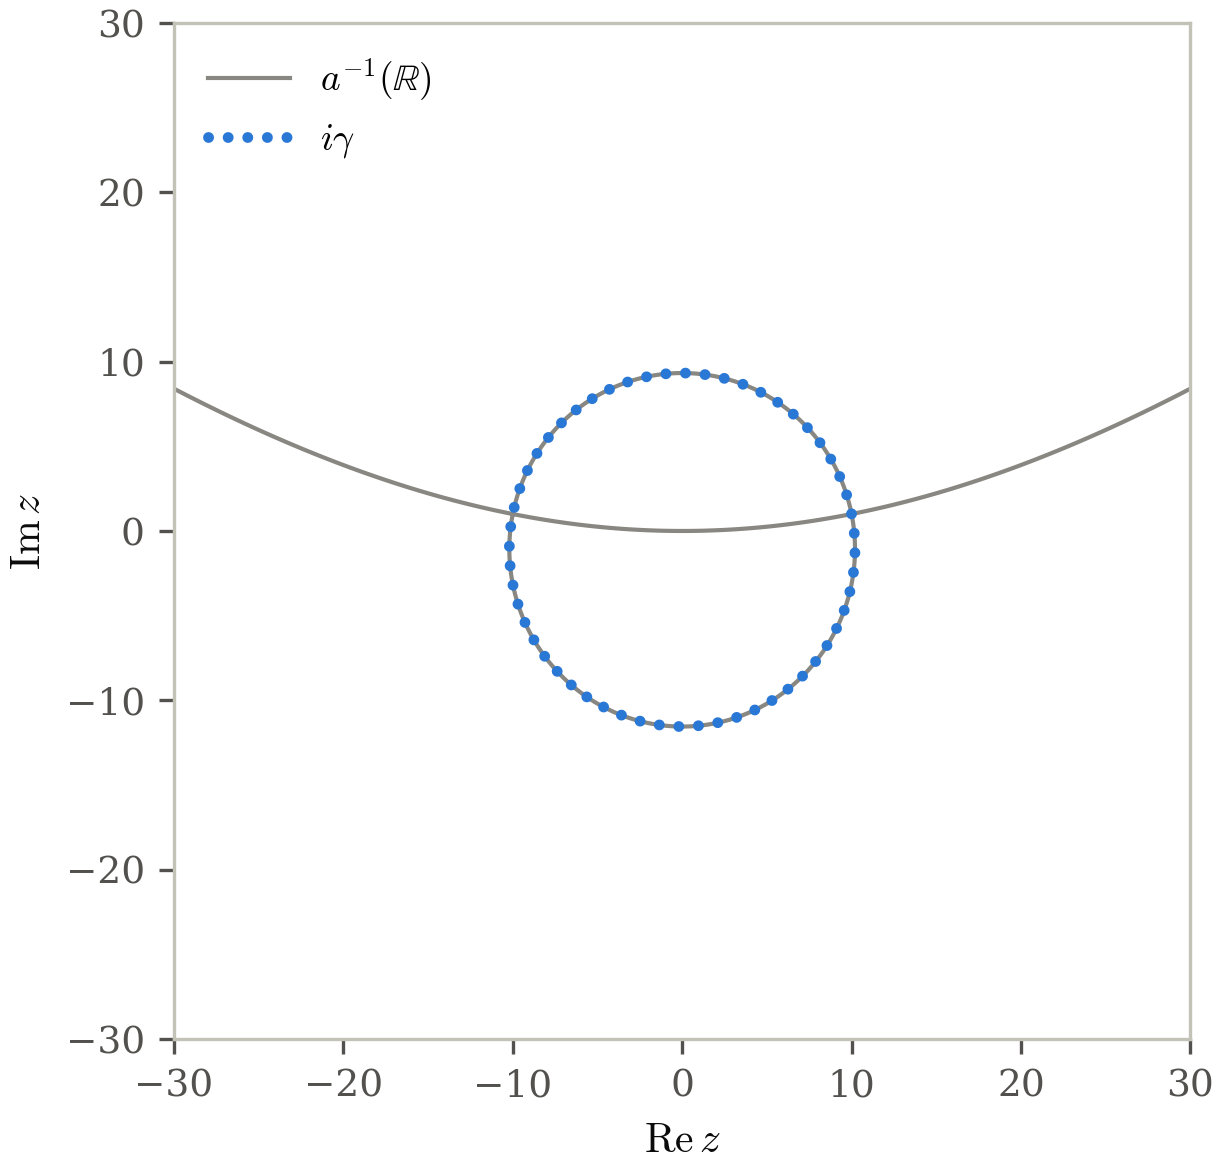
\includegraphics[width=\textwidth]{figures/fig_preimage_real_a.png}
         \caption{Preimage of $\R$}
         \label{fig:Second1}
     \end{subfigure}
     \hfill
     \begin{subfigure}[b]{0.45\textwidth}
         \centering
         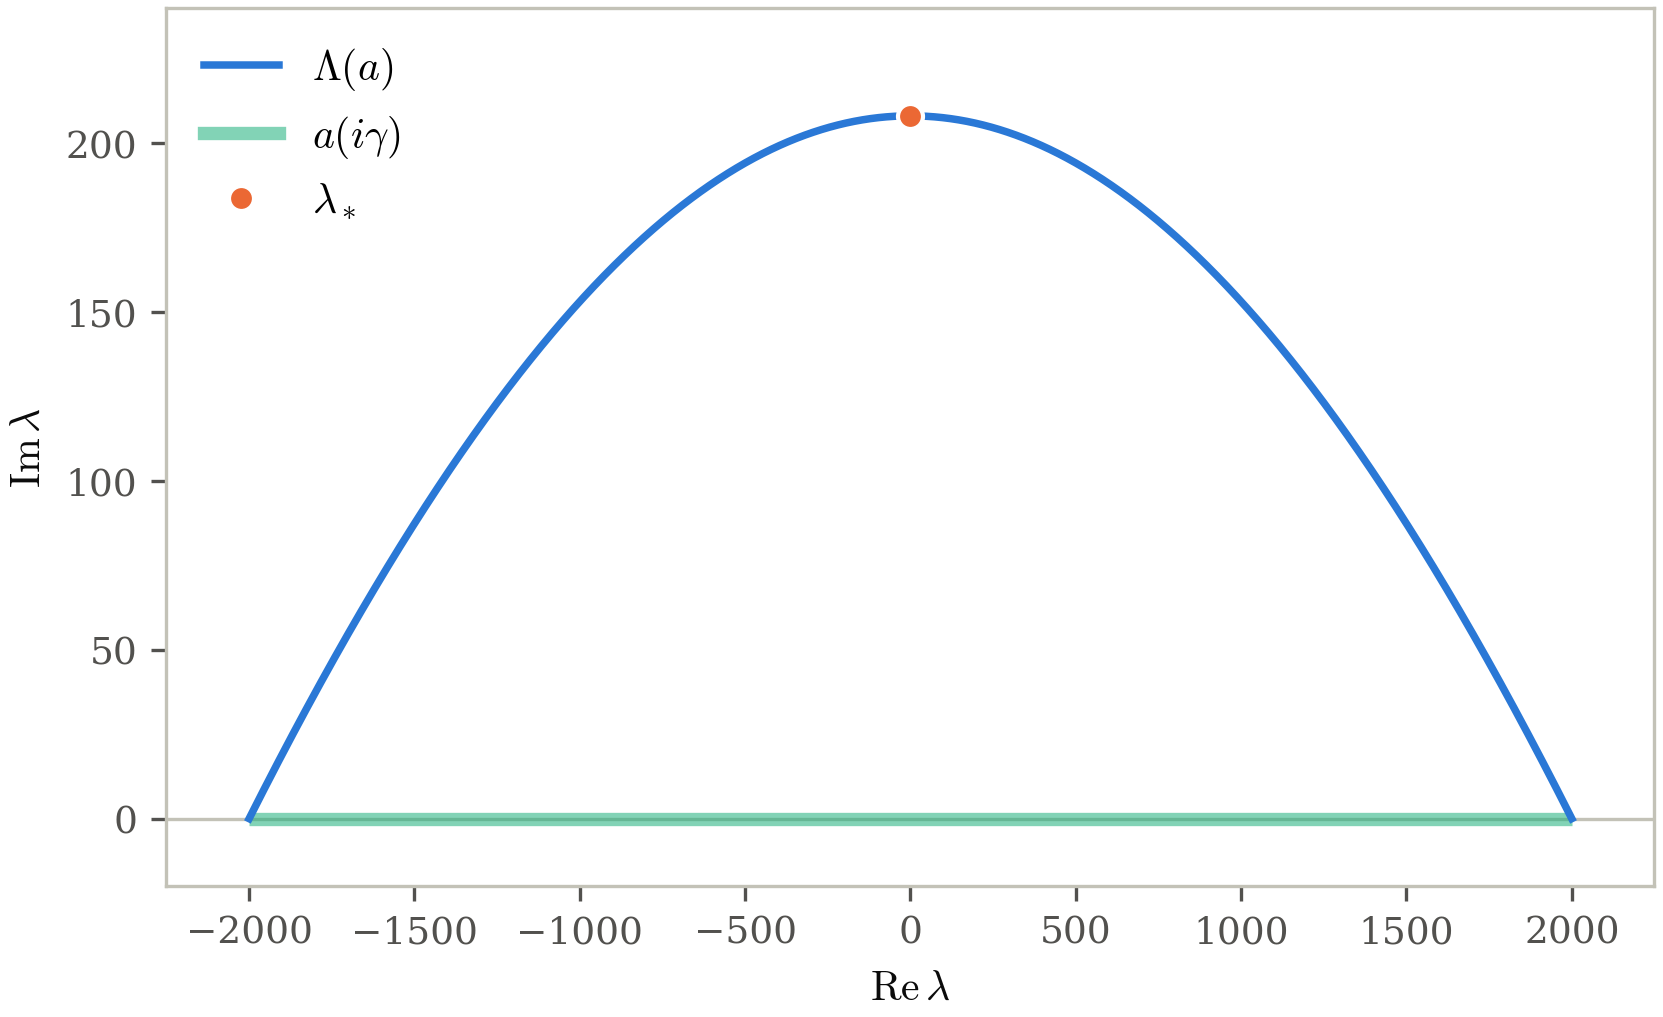
\includegraphics[width=\textwidth]{figures/fig_limiting_spectrum_a.png}
         
         \caption{Limiting spectrum}
         \label{fig:Second2}
     \end{subfigure}

     \vspace{1em} % Adds some vertical spacing between the rows

     % --- SECOND ROW ---
     \begin{subfigure}[b]{0.45\textwidth}
         \centering
         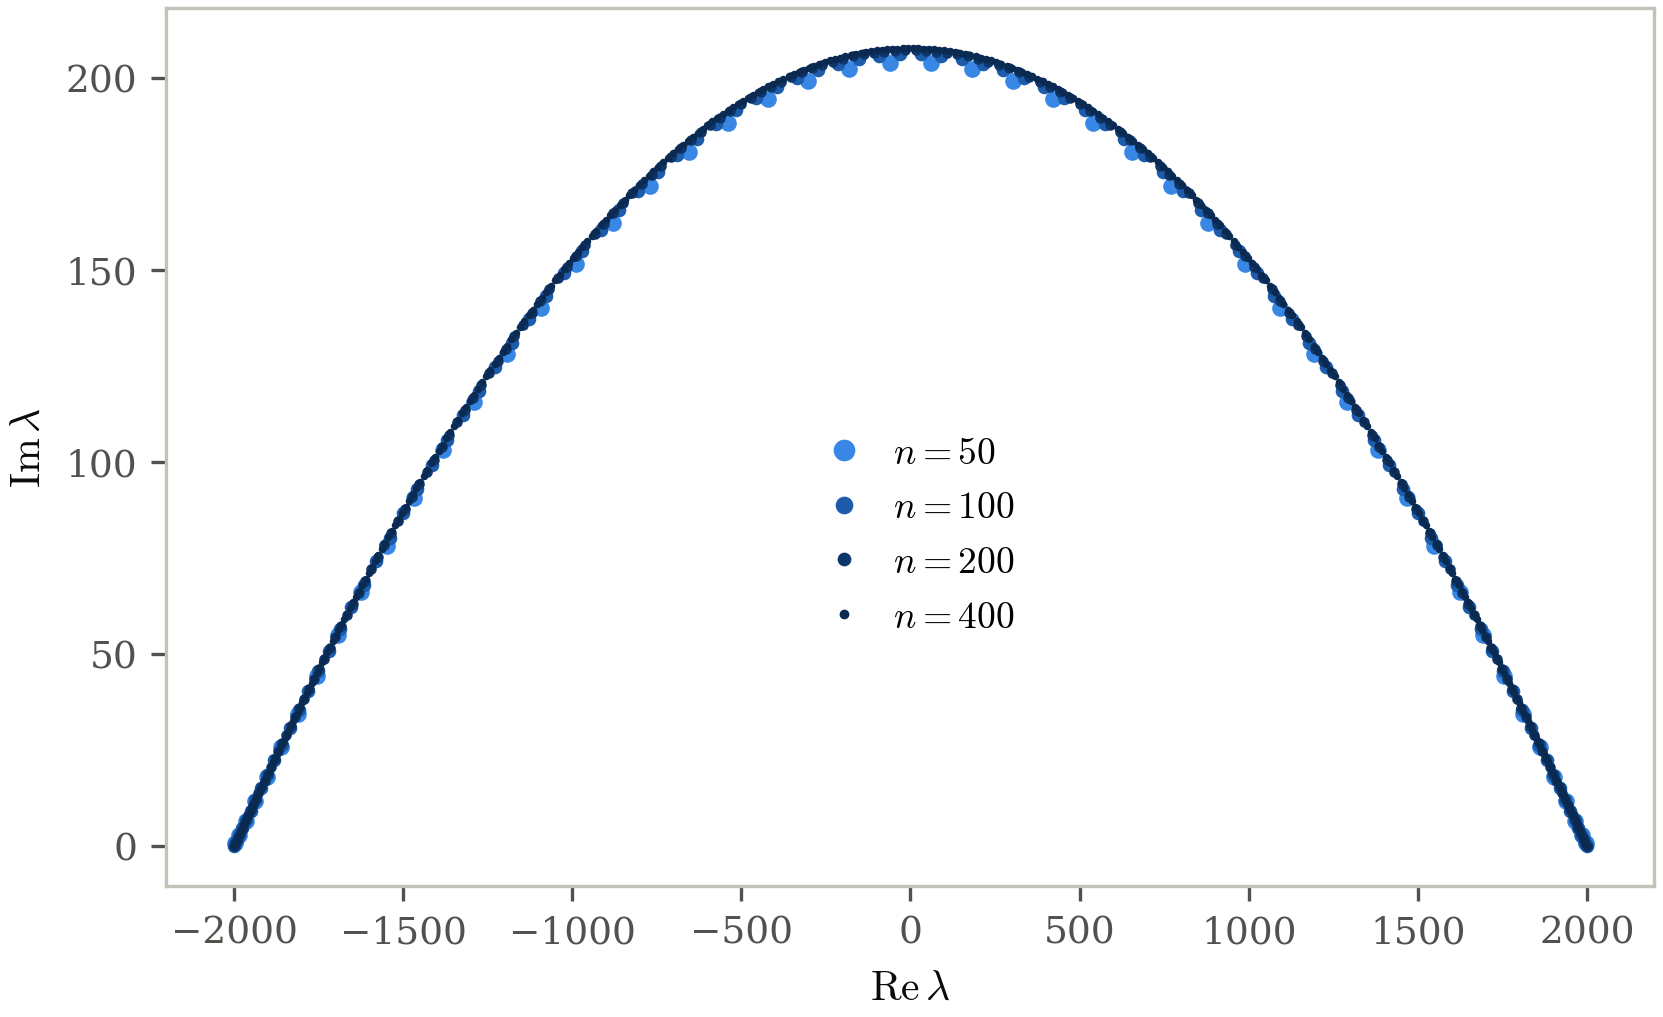
\includegraphics[width=\textwidth]{figures/fig_finite_spectra_a.png}
         \caption{Finite section spectra}
         \label{fig:Second3}
     \end{subfigure}
     
     \caption{Preimage of $\R$ and Limiting Spectrum for $a$ as in Proposition \ref{prop:complex}}
     \label{fig:Second}
\end{figure}

% \section{Topological root counts versus modulus ordering}
% \label{sec:topology}

% The counterexamples do not invalidate the root count suggested by the argument principle. They invalidate the additional radial ordering that one might try to infer from it. We first state the root count in a form that does not require a smooth boundary.

% \begin{proposition}
% \label{prop:root-count}
% Let \(f(z)=\sum_{k=-r}^{s}f_kz^k\), with \(f_{-r}f_s\neq0\), and let \(\Gamma\subset\C\setminus\{0\}\) be a positively oriented Jordan curve satisfying
% \[
%  f(\Gamma)\subset\R,\qquad\wind(\Gamma,0)=1.
% \]
% For every \(\lambda\notin\R\), exactly \(r\) roots of \(z^r(f(z)-\lambda)\) lie in the bounded interior of \(\Gamma\), counted with multiplicity.
% \end{proposition}

% \begin{proof}
% Write the polynomial factorization as
% \[
%  f(z)-\lambda=f_s z^{-r}\prod_{j=1}^{r+s}(z-\zeta_j).
% \]
% No \(\zeta_j\) lies on \(\Gamma\), because \(\lambda\notin\R\). The loop \(f\circ\Gamma\) lies in \(\R\), and hence has winding number zero about \(\lambda\). Additivity of winding number under multiplication gives
% \[
%  0=\wind(f\circ\Gamma,\lambda)
%    =-r\wind(\Gamma,0)
%        +\sum_{j=1}^{r+s}\wind(\Gamma,\zeta_j).
% \]
% For a positively oriented Jordan curve, each summand is \(1\) for an interior root and \(0\) for an exterior root. The sum is therefore \(r\). This proof uses winding numbers of continuous loops only; no rectifiability assumption is needed.
% \end{proof}

% For the symbol \(b=h^2\), Proposition~\ref{prop:root-count} gives two roots inside \(\gamma\) for each nonreal parameter. Nevertheless, one interior root and one exterior root can be the equal-modulus middle pair.

% \begin{proposition}
% \label{prop:sides}
% Let \(D\) be the bounded interior of the curve \(\gamma\) in Proposition~\ref{prop:curve}. Then
% \begin{equation}
%  -\rho\in D,\qquad \rho\notin\overline D.
%  \label{eq:opposite-sides}
% \end{equation}
% These inside--outside assignments persist for the branches \(v(\lambda)\) and \(u(\lambda)\), respectively, near \(\lambda_0\), including at the nonreal points of the spectral arc \eqref{eq:arc-param}.
% \end{proposition}

% \begin{proof}
% If \(z\in\gamma\cap\R\), then \(h(z)\) is both real, because \(h\) has real coefficients, and purely imaginary, by \eqref{eq:gamma}. Thus \(h(z)=0\). Conversely, every zero of \(h\) in \(|z|<30\) belongs to \(\gamma\).

% Let \(p(z)=P_0(z)=zh(z)\). Its values satisfy
% \[
%  p(-30)=47009>0,\qquad p(-\rho)=-L\rho<0,
% \]
% \[
%  p(0)=-10201<0,\qquad p(\rho)=L\rho>0.
% \]
% Hence \(p\) has roots \(\eta_-\) and \(\eta_+\) with
% \begin{equation}
%  \eta_-\in(-30,-\rho),\qquad \eta_+\in(0,\rho).
%  \label{eq:eta}
% \end{equation}
% Lemma~\ref{lem:rouche} shows that these are exactly the two roots inside \(|z|<30\). Consequently,
% \[
%  \gamma\cap\R=\{\eta_-,\eta_+\}.
% \]
% The open interval \((\eta_-,\eta_+)\) contains \(0\) and does not meet \(\gamma\). Since \(0\in D\), this whole interval lies in \(D\). Each exterior real ray lies in the unbounded complementary component, because it is connected, avoids \(\gamma\), and reaches arbitrarily large modulus. The inequalities \eqref{eq:eta} therefore imply \eqref{eq:opposite-sides}.

% The points \(\pm\rho\) do not lie on \(\gamma\), so sufficiently small neighborhoods of them remain on their respective sides. Continuity of \(u\) and \(v\) proves the final assertion.
% \end{proof}

% At the nonreal parameters \(\lambda(t)\), the two equal-modulus roots thus lie on opposite sides of \(\gamma\), while Lemma~\ref{lem:ordering} and continuity place them at ranks \(2\) and \(3\). The prospective inference
% \[
%  \text{interior roots have smaller modulus than exterior roots}
% \]
% is therefore false even for a real-analytic Jordan curve and a symbol with real coefficients. The failure does not depend on a multiple root of the spectral polynomial or on ambiguity involving additional equal-modulus roots.

% For comparison, a concentric circle supplies precisely the radial information absent from a general Jordan curve.

% \begin{corollary}
% \label{cor:circle}
% Suppose that a Laurent polynomial \(f\), with pole order \(r\geq1\) at \(0\), is real-valued on \(|z|=R\) for some \(R>0\). Then, for every \(\lambda\notin\R\), its modulus-ordered roots satisfy
% \[
%  |z_r(\lambda)|<R<|z_{r+1}(\lambda)|.
% \]
% In particular, \(\Lambda(f)\subset\R\).
% \end{corollary}

% \begin{proof}
% No root lies on \(|z|=R\) when \(\lambda\notin\R\). Proposition~\ref{prop:root-count} gives exactly \(r\) roots in the disk, which proves the strict inequalities. The conclusion follows from \eqref{eq:SS}.
% \end{proof}

% \section{Conclusion}

% We  have provided two simple counter examples to a well-known conjecture on the reality



% The right-to-left implication in \eqref{eq:question} is false. The explicit real-coefficient symbol \(b=h^2\) admits a real-valued, real-analytic Jordan curve around \(0\), but its limiting spectrum contains a regular arc crossing the real axis at \(\lambda_0=(20192/97)^2\). The four-diagonal symbol \(a\) in \eqref{eq:a-intro} gives an explicit nonreal limiting spectral point.

% The distinction is between a topological partition and an ordering by Euclidean modulus. The curve fixes the number of interior roots, but that partition need not agree with the partition into the \(r\) smallest roots and the remaining \(s\) roots. Any sufficient criterion of this type must add a condition that excludes this mismatch. The constructions address the sufficiency direction only; no conclusion against the reverse implication is drawn.

\section*{Acknowledgment}
The counterexamples and a first draft of this paper were
produced by GPT-6 Astra Pro (OpenAI) in sessions directed by F. Rohner. C. Thalhammer used Opus 5 (Anthropic) to produce Figures \ref{fig:Main} and \ref{fig:Second}. All mathematical content has been
verified independently by the authors, and the authors take full
responsibility for the content.
\printbibliography

\end{document}
